\subsection{Kommunikationsprotokoll}\label{Protokoll}
\subsubsection{Projektteilbereich Übersicht}
Für die Kommunikation zwischen dem FPGA und dem UserInterface wurde ein spezielles Protokoll entwickelt, welches auf UART aufbaut. Ziel ist ein schnelles Senden der Messdaten und Austauschen der Konfiguration mit inkludierter Fehlerdetektion. Das gesamte Protokoll ist aufgebaut aus einzelnen Daten mit einer Wortlänge von 12-Bit, was die Handhabung der 12-Bit-ADC-Messwerte vereinfacht und praktisch für größere Zahlen ist. Dass mit UART  auf unterer Ebene jeweils 8 Bit gesendet werden, wird ignoriert und ist für die höheren Ebenen irrelevant. Es werden immer Pakete mit einem idententischen Aufbau gesendet.
\subsubsection{Paketspezifikation FPGA zu UserInterface}
\begin{figure}[!h]
\begin{center}
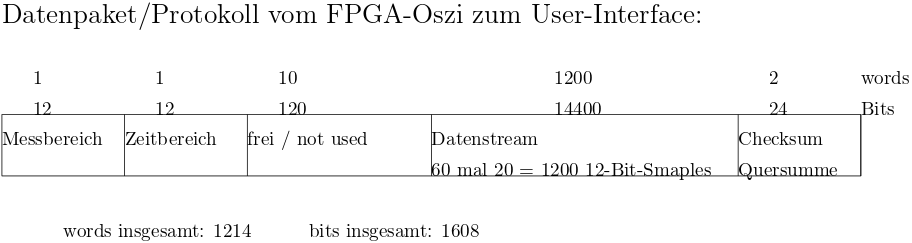
\includegraphics[width=15cm]{SAUER/Grafiken/Kommunikationsprotokoll/Datenstreampaket.png}
\caption{Paketspezifikation FPGA zu UserInterface}
\label{Datenstreampaket}
\end{center}
\end{figure}
\subsubsection{Paketspezifikation UserInterface zu FPGA}
\begin{figure}[h]
\begin{center}
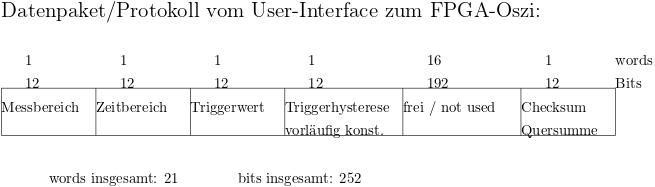
\includegraphics[width=15cm]{SAUER/Grafiken/Kommunikationsprotokoll/Controllerpaket.png}
\caption{Paketspezifikation UserInterface zu FPGA}
\label{Controllerpaket}
\end{center}
\end{figure}
\subsubsection{Messbereichseinstellung}
Der Messbereich wird über diesen Wert eingestellt. Das FPGA-Oszilloskop bekommt diesen vom UserInterface vorgegeben und schickt diesen zur Kontrolle mit den Messwerten auch wieder zurück. In der folgenden Tabelle sind die durchnummerierten Messbereiche zu finden.
\begin{tabular}[h]{l|l} %l = left c = center r = right
	Wert / Nummer& Messbereich\\
	\hline\hline
	0 & 1 : 1 (beispiel)\\
	\hline
	1 & 1 : 10 (beispiel)\\
	\hline
	2 & 1 : 24  (beispiel)\\
\end{tabular}
\subsubsection{Zeitbereichseinstellung}\label{Zeitbereichseinstellung}
Die Zeitbereichseinstellung bezieht sich auf einen Zeitabschnitt (Division). Davon sind immer zehn in der Grafik im UserInterface zu sehen, ein Raster sozusagen. So wie bei den alten, analogen Oszilloskopen, bei denen auch ein Raster am Bildschirm zu sehen war. Hat ein Zeitabschnitt beispielsweise eine Dauer von 20ms, so sind in der Anzeige insgesamt 200ms abgebildet.\\Um die große, unilineare Spanne von Zeitbereichen mit 12 Bit abzudecken, hat die Projektgruppe hier eine Wertetabelle geplant.\\
\begin{tabular}[h]{l|l||l|l} %l = left c = center r = right
	Wert / Nummer& Zeitbereich & Wert / Nummer& Zeitbereich\\
	\hline\hline
	0 & 2 $\mu$s & 12 & 5 ms\\
	\hline
	1 & 5 $\mu$s & 13 & 10 ms\\
	\hline
	2 & 10 $\mu$s & 14 & 20 ms\\
	\hline
	3 & 10 $\mu$s & 15 & 50 ms\\
	\hline
	4 & 20 $\mu$s &16 & 100 ms\\
	\hline
	5 & 50 $\mu$s &17 & 200 ms\\
	\hline
	6 & 100 $\mu$s &18 & 500 ms\\
	\hline
	7 & 200 $\mu$s & 19 & 1 s\\
	\hline
	8 & 500 $\mu$s & 20 & 2 s\\
	\hline
	9 & 1 ms  & 21 & 5 s\\
	\hline
	10 & 2 ms & 22 & 10 s\\
	\hline
	11 & 5 ms & & \\
\end{tabular}
\subsubsection{Messdaten}
Die Samples werden direkt aus dem Buffer als Bit-Stream zum UserInterface geschickt. Dieses trennt die Samples anschließend wieder durch zählen, alle 12 Bit beginnt ein neuer Messwert. Es werden immer genau 1200 Messwerte chronologisch (frühester Messwert zuerst, MSB voran)geschickt, da eine Genauigkeit von 20 Samples pro Zeitabschnitt festgelegt ist und immer 60 Zeitabschnitte gesendet werden. 60 mal 20 Samples mal 12 Bit ergibt eine Gesamtanzahl von 14400 Bits.
\subsubsection{Checksum}
Die sogenannte "Checksum" ist die Quersumme des gesamten, bisher gesendeten Datenpakets. Alle logischen Einser werden addiert und als Checksum mitgesendet. So können Übertragungsfehler mit hoher Wahrscheinlichkeit festgestellt werden. Die Quersumme kann vom UserInterface zum FPGA maximal 240 betragen und umgekehrt maximal 14544. Beide der Kontrollzahlen setzten sich aus 2 Wortlängen zusammen, somit 24 Bit.
\subsubsection{frei / not used}
Diese Abschnitte werden (noch) nicht benutzt und dienen für spätere, eventuelle Erweiterungen. Eine zusätzliche Spektralanalyse-Funktion könnte die freien Wörter nutzen.
